\documentclass[a4paper, 12pt]{report}
\usepackage[spanish]{babel}
\usepackage[utf8]{inputenc}
\usepackage{textcomp}
\usepackage{booktabs}
\usepackage{amssymb}
\usepackage{bussproofs}

\usepackage{fancyhdr}
\usepackage{graphicx}
\usepackage{amsmath}

\pagestyle{fancy}
\lhead{Almeida, Figueroa \& Ibarra}
\chead{Tarea 1}
\rhead{\today}
\begin{document}
	\begin{enumerate}
		\item Explica el concepto de agregación en el modelo E/R y
		 proporciona un par de ejemplos.\\

		 Es un concepto de abstracción, permite construir entidades
		 de más alto nivel compuestas a partir de otras más pequeñas.\\
		\textbf{Ejemplo1:}\\
		Un científico puede trabajar en varios proyectos y un proyecto
		tiene como participante a varios científicos. Además un
		científico pública un artículo sobre el proyecto en el que
		trabajo.\\
		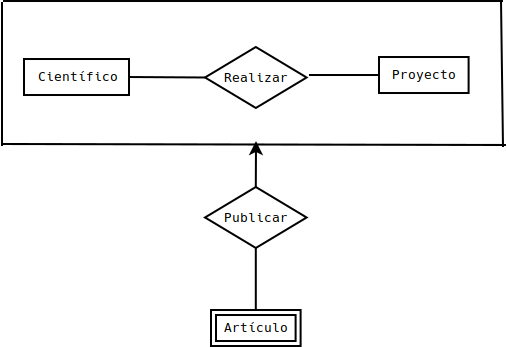
\includegraphics[scale= 0.5]{Ejemplo1}\\
		\textbf{Ejemplo2:}\\
		Un empleado trabaja en un departamento en una sucursal, la
		sucursal, los departamentos y el empleado es dirigido por un
		director.\\
		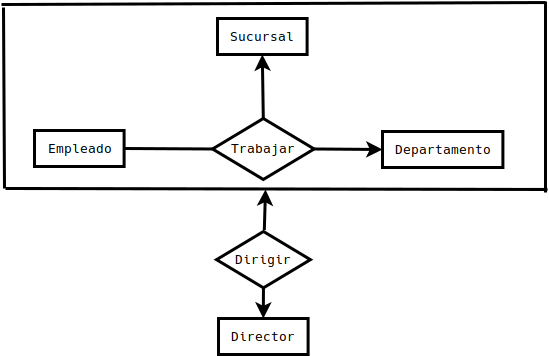
\includegraphics[scale= 0.5]{Ejemplo2}
		\item \textbf{Ingeniería inversa}:
		Una compañía celular requiere una base de datos para realizar
		un seguimiento de sus clientes, sus planes de suscripción y
		los teléfonos móviles que  están  utilizando.  El diagrama
		E/R de  la  siguiente figura  muestra  entidades  de  interés
		para  la  compañía  y  las  relaciones  entre  ellas.
		Tomando  como base el esquema proporcionado, responde a las
		siguientes preguntas justificando tu respuesta. Para cada
		pregunta, identificar el o los elementos en el diagrama E/R
		que utilizaste para tu respuesta. En caso de que alguna
		pregunta no se cumpla en el diagrama actual, indica las
		modificaciones que deberían hacerse para que se permita dicho
		comportamiento.\\
		\begin{enumerate}
			\item ¿Un cliente puede tener un número ilimitado de planes?\\
			Sí, ya que la relación de poseer es de muchos a muchos, por
			lo que un cliente puede tener más de un plan.
			\item ¿Un cliente puede existir sin un plan?\\
			Sí, ya que la relación de poseer, no es total del lado del
			cliente, por lo que no es necesario que tenga un plan.
			\item ¿Es posible crear un plan sin saber quién es el
			cliente?\\
			No, la relación que va desde el plan hasta poseer es total,
			es decir un plan siempre tiene un cliente, por lo que es
			necesario que se sepa quién es el cliente al que va
			dirigido.
			\item ¿El operador quiere limitar los tipos de dispositivos
			que se pueden vinicular a un tipo de plan específico?\\
			Sí, ya que un teléfono incluye solo un plan.
			\item ¿Es posible mantener los datos relativos a un
			teléfono, sin conectarlo a un plan?\\
			Sí, ya que la participación de un teléfono a incluir no es
			total, por lo que el teléfono no necesita tener un plan.
			\item ¿Puede un teléfono asociar varios planes?\\
			No, no puede, ya que la relación incluir es uno a muchos,
			es decir un plan puede incluir varios teléfonos pero un
			teléfono solo puede tener un plan.
			\item Supongamos que existe un tipo de teléfono que puede
			utilizar múltiples sistemas operativos. ¿Este tipo de
			situación podría tener cabida dentro del modelo incluido
			en la figura?\\
			Sí, solo se necesitaría cambiar la relación de tener que va
			desde tipo de teléfono a sistema operativo a una relación
			muchos a muchos
			\item ¿La empresa capaz de realizar un seguimiento de un
			fabricante sin mantener información sobre sus teléfonos?\\
			No, no puede, ya que desde el cliente o desde el plan,
			no se puede identificar al fabricante ya que no están
			relacionados, para identificar el fabricante, se necesitan
			los datos del teléfono.
			\item ¿Puede el mismo sistema operativo utilizarse en
			múltiples tipos de dispositivos?\\
			Sí, ya que la relación tener entre tipo de teléfono y
			sistema operativo es muchos a uno, es decir, un sistema
			operativo puede estar en varios tipos de teléfonos, pero
			un tipo de teléfono sólo tiene un sistema operativo.
			\item Hay dos relaciones entre el Cliente y el Plan. Explicar en qué difieren.\\
			Poseer es una relación con cardinalidad muchos a muchos,
			además tiene participación parcial de parte del cliente y
			total de parte del plan.\\
			Administrar es una relación de uno a muchos con
			participación total de los dos lados.
			\item Caracterizar el grado y la cardinalidad de la
			relación que une al cliente a sí mismo. Explicar su
			significado.\\
			Tiene cardinalidad uno a muchos con participación total de
			un lado y parcial del otro, es decir un cliente tiene muchos clientes pero un cliente solo tiene un cliente,
			además un cliente siempre tiene un cliente y a la vez un
			cliente puede no tener un cliente.
			\item ¿Es posible vincular un teléfono a un cliente
			específico en un plan con múltiples clientes?\\
			Sí, ya que un plan es administrado solo por un cliente.
			\item ¿Puede la compañía rastrear un teléfono sin identificar su sistema operativo?\\
			Sí ya que no depende del sistema operativo, hay otras
			formas de identificar un teléfono.

		\end{enumerate}

	\end{enumerate}
\end{document}
